\documentclass[8pt, aspectratio=169]{beamer}
\usepackage[utf8]{inputenc}
\usepackage[russian]{babel}
\usepackage{amsmath, amssymb, amsfonts}
\usepackage{graphicx}
\usepackage{hyperref}
\usepackage{xcolor}
\usepackage{wrapfig}
\usepackage{float}
\usepackage{gensymb}
\usepackage{textcomp}
\usepackage{multirow}

% Настройка цвета формул
\definecolor{mathcolor}{RGB}{139,69,19} % brown
\definecolor{darkgreen}{RGB}{0,100,0} % темно-зеленый (dark green)
\everymath{\color{mathcolor}}
\everydisplay{\color{mathcolor}}
\linespread{1.2}

% Настройка темы Beamer
\usetheme{Madrid}
\usecolortheme{default}

% Убираем навигационные символы
\setbeamertemplate{navigation symbols}{}

% Определение команд
\newcommand{\Def}{{\color{darkgreen}\boxed{\color{darkgreen}\mathbf{Def:}}}}
\newcommand{\Th}[1]{{\color{darkgreen}\boxed{\color{darkgreen}\mathbf{Th~#1:}}}}
\newcommand{\St}[1]{{\color{darkgreen}\boxed{\color{darkgreen}\mathbf{Statement~#1:}}}}
\newcommand{\Cons}{{\color{darkgreen}\boxed{\color{darkgreen}\mathbf{Cons:}}}}
\newcommand{\Ex}[1]{{\color{darkgreen}\boxed{\color{darkgreen}\mathbf{Example~#1:}}}}
\newcommand{\Disc}{{\color{darkgreen}\boxed{\color{darkgreen}\mathbf{Discussion:}}}}

\title{1.4 Натуральные числа. Делимость. Простые числа. Бесконечность множества простых чисел.}
\author{}
\institute{}
\date{}

\begin{document}

\begin{frame}
\titlepage
\end{frame}

\begin{frame}{\textbf{Определение натуральных чисел}}
$\Def$ \textbf{Натуральные числа} - числа, возникающие естественным образом при счёте предметов,

т.е. $1, 2, 3, ...$

Изучением свойств целых чисел и в частности натуральных и простых занимается \textbf{теория чисел}

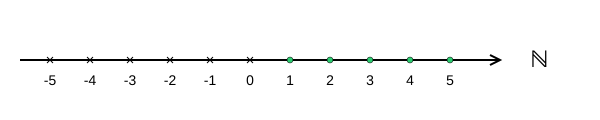
\includegraphics[width=0.6\textwidth]{./images/N_numbers.png}

Их обозначают символом $\mathbb{N}$
\begin{gather*}
    \mathbb{P} \subset \mathbb{N} \subset \mathbb{N}_0 \subset \mathbb{Z} \subset \mathbb{Q} \subset \mathbb{R} \subset \mathbb{C} \\
    \mathbb{Z}^{-}\cup \{0\} \cup \mathbb{Z}^{+} = \mathbb{Z}^{-}\cup \mathbb{N}_0 = \mathbb{Z} \\
    \mathbb{Z}^{+} = \mathbb{N} \\
    \mathbb{Q}\;\cup\;\mathbb{I} = \mathbb{R}
\end{gather*}

В некоторых книгах натуральными числами считают $0, 1, ...$

Например: Торенс Тао "Математический анализ"

\end{frame}

\begin{frame}{\textbf{Определение множества N через аксиомы Пеано}}
Есть строгое определение через \textbf{аксиомы Пеано}:
\begin{enumerate}
\item $1 \in \mathbb{N}$
\item $x \in \mathbb{N} \Rightarrow S(x) \in \mathbb{N}$
\item $\nexists x \in \mathbb{N}: S(x) = 1$
\item $(S(b) = a\; \land \; S(c) = a) \Rightarrow b = c$
\item $P(1) \land \forall{n}{\color{darkgreen}(P(n) \Rightarrow P(S(n)))} \Rightarrow \forall{n}\in \mathbb{N} (P(n))$
\end{enumerate}

Определение сложения:
\begin{enumerate}
\item База $a + 1 = S(a)$
\item Переход: $a + S(b) = S(a + b)$
\end{enumerate}
\end{frame}

\begin{frame}{\textbf{Операции на множестве N:}}
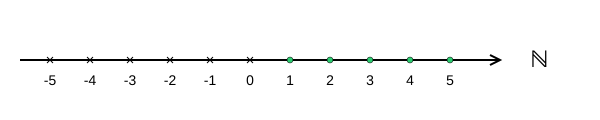
\includegraphics[width=0.8\textwidth]{./images/N_numbers.png}

[$\checkmark$]: $a + b = c$, где $a, b, c \in \mathbb{N}$

[$\times$]: $a - b = c$, где $a, b, c \in \mathbb{N}$, но только при $a > b$

[$\checkmark$]: $a \cdot b = c$, где $a, b, c \in \mathbb{N}$

[$\times$]: $a/b = c$, где $a, b \in \mathbb{N} \iff a \mathbin{\vdots} b$

[$\times$]: $\sqrt{a} = c$, где $a, c \in \mathbb{N} \iff a = c^2, \; c \in \mathbb{N}$

Т.к. множество $\mathbb{N}$ - чисел строго упорядоченно, и имеют место отношения порядка и эквивалентности:

$<, >, \le, \ge, =$

\begin{enumerate}
\item $a < b \land b < c \Rightarrow a < c$
\end{enumerate}

\end{frame}

\begin{frame}{\textbf{Делимость}}
$\Def$ Если $a/b = q: \; a, b, q \in \mathbb{N}$, то говорят, что:

$a$ \textbf{делится на} $b$ или, что $b$ \textbf{делит} $a$,

при этом $a$ называется \textbf{кратным} числа $b$, а $b$ - \textbf{делителем} числа $a$ и обозначается:

$b\setminus a$ или $a \mathbin{\vdots} b$

\vspace{1.0cm}

$\Ex{}$

\begin{enumerate}
    \item Для $\mathbb{N}$ - чисел: $21 = 7\cdot3$
    \item Для $\mathbb{Z}$ - чисел: $0 = 9\cdot 0$
\end{enumerate}
\end{frame}

\begin{frame}{\textbf{Делимость}}
$\Th{1}$ Если $a \mathbin{\vdots} m \land m \mathbin{\vdots} b \Rightarrow a \mathbin{\vdots} b$

$\square$

$a=ma_1 \land m = bm_1 \Rightarrow a = bm_1a_1 \Rightarrow a \mathbin{\vdots} b$

$\blacksquare$

$\Th{2}$ Если в равенстве вида $k + l + ... + n = p + q + ... + s$ относительно всех членов, кроме какого-либо одного, известно, что они кратны $b$, то и этот один член кратен $b$

$\square$

Пусть этим одним членом будет $k$, тогда:
\begin{gather*}
l = b \cdot l_1, ..., n = b \cdot n_1, p=b \cdot p_1, q=b \cdot q_1, ..., s=b \cdot s_1 \\
\Downarrow \\
k = (p + q + ... + s) - (l + ... + n) = b \cdot (p_1 + q_1 + ... + s_1) - b \cdot (l_1 + ... + n_1) \\
\Downarrow \\
k = b\cdot k_1, k_1 \in \mathbb{N} \Rightarrow k \in \mathbb{N}
\end{gather*}

$\blacksquare$

\end{frame}

\begin{frame}{Делимость}
$\Th{3}$ Всякое целое $a$ представляется единственным способом
с помощью положительного целого $b$ следующим равенством:

\[
a = bq + r, \quad 0 \le r < b \qquad (1)
\]

$\square$ от противного

Пусть имеется другое представление числа $a$:
$a = bq_1 + r_1, \quad 0 \le r_1 < b \qquad (2)$

Вычтем $(2)$ из $(1)$:

$0 = b(q - q_1) + (r - r_1)$

Т.к. первое слагаемое кратно $b$, т.е. $b(q - q_1)\mathbin{\vdots} b$

а $0$ тоже кратен $b$, то следует что $(r - r_1) \mathbin{\vdots} b$, это следует из $\Th{2}$

Но мы знаем, что $0 \le r < b, 0 \le r_1 < b$, а это значит, что:

$r - r_1 = 0 \Rightarrow r = r_1 \Rightarrow q - q_1 = 0 \Rightarrow q = q_1$

противоречие

$\blacksquare$
\end{frame}

\begin{frame}{Делимость}
Итак, мы выяснили, что число $a$ можно представить следующим образом (и притом единственно):
\[
a = bq + r, 0 \le r < b
\]

$\Def$ Число $q$ называется \textbf{неполным частным}, а число $r$ - остатком от деления $a$ на $b$

$\Def$ Если $r = 0$, то $q$ называют просто \textbf{частным}

$\Ex{}$ $64 = 4\cdot 16 + 0, \quad 177 = 14 \cdot 12 + 9$

В контексте $\mathbb{N}$ чисел: $64 = 4\cdot 16$
\end{frame}

\begin{frame}{\textbf{Наибольший общий делитель} (НОД)}
$\Def$ Всякое $\mathbb{N}$ число делящее одновременно числа $a, b, ... $ называется их \textbf{общим делителем},

и наибольший из них называется \textbf{НОД} и обозначается:

\begin{gather*}
(a, b, ...) \\
\text{НОД}(a, b, ...) \\
\gcd(a, b, ...)
\end{gather*}

$\Def$ Если $\text{НОД}(a, b, ...) = 1$, то совокупность чисел $a, b, ...$ называют \textbf{взаимно простыми}.

$\Ex{}$ $\text{НОД}(6, 10, 15) = 1$

$\Def$ Если каждая пара чисел из совокупности $a, b, ...$ взаимнопроста, то такие числа называют \textbf{попарно простыми}.

$\Ex{}$ $\text{НОД}(8, 13, 21) = \text{НОД}(8, 13) = \text{НОД}(13, 21) = \text{НОД}(8, 21) = 1$

\end{frame}

\begin{frame}{\textbf{Делимость}}
\begin{enumerate}
\item Если $a \mathbin{\vdots} b$, то совокупность общих делителей чисел $a$ и $b$ совпадают с совокупностью делителей числа $b$

\item Если $a = bq+c$, то совокупность общих делителей чисел $a$ и $b$ совпадает с совокупностью общих делителей чисел $b$ и $c$ и $\text{НОД}(a, b) = \text{НОД}(b, c)$

$\square$ из $\Th{2}$ $\blacksquare$

\item Для поиска $\text{НОД}$ применяется алгоритм Евклида:

\begin{aligned} a &= bq_1 + r_2, & 0 < r_2 < b, \\
    b &= r_2q_2 + r_3, & 0 < r_3 < r_2, \\
    r_2 &= r_3q_3 + r_4, & 0 < r_4 < r_3, \\
    . & . . . . . . . & . . . . . . \\
    r_{n-2} &= r_{n-1}q_{n-1} + r_n, & 0 < r_n < r_{n-1}, \\
    r_{n-1} &= r_n q_n,
\end{aligned}

\end{enumerate}
\end{frame}

\begin{frame}{\textbf{Свойства НОД}}
\begin{enumerate}
\setcounter{enumi}{3}
\item Совокупность общих делителей чисел $a$ и $b$ совпадает с совокупностью делителей их общего наибольшего делителя, т.е. $\text{НОД}$.

Этот $\text{НОД}$ равен последнему не равному нулю остатку алгоритма Евклида

\vspace{0.5cm}

$\Ex{}$

\begin{gather*}
\text{НОД}(525, 231) = ? \\
525 = 231 \cdot {\color{darkgreen}\boxed{\color{darkgreen}2}} + 63 \\
231 = 63 \cdot {\color{darkgreen}\boxed{\color{darkgreen}3}} + 42 \\
63 = 42 \cdot {\color{darkgreen}\boxed{\color{darkgreen}1}} + 21 \\
42 = {\color{blue}\boxed{\color{blue}21}} \cdot {\color{darkgreen}\boxed{\color{darkgreen}2}} \\
\text{НОД}(525, 231) = 21
\end{gather*}

\end{enumerate}
\end{frame}

\begin{frame}{\textbf{Свойства НОД}}
\begin{enumerate}
\setcounter{enumi}{4}
\item $\text{НОД}(am, bm) = m\cdot \text{НОД}(a, b)$

\item Пусть $d$ - любой общий делитель чисел $a$ и $b$, тогда справедливо:
\[
\text{НОД}\left(\frac{a}{d}, \frac{b}{d}\right) = \frac{\text{НОД}(a, b)}{d}
\]

\item Если $\text{НОД}(a, b) = 1 \Rightarrow \text{НОД}(ac, b) = \text{НОД}(c, b)$
\item Если $\text{НОД}(a, b) = 1 \land ac\mathbin{\vdots}b \Rightarrow c \mathbin{\vdots} b$
\end{enumerate}
\end{frame}

\begin{frame}{\textbf{Цепные дроби и НОД}}
$\Disc$ Интересно, что:
\[
\frac{525}{231} = {\color{darkgreen}[2, 3, 1, 2]} = 2 + {\frac{1}{3 + \frac{1}{1 + \frac{1}{2}}}}
\]
На самом деле алгоритм Евклида применяется не только для вычисления $НОД(a, b)$, но и для построения цепных дробей для любого $\mathbb{R}$ - числа.

\textbf{Цепная дробь} - это инструмент для выражения (приближения) $\mathbb{I}$ - чисел в конечной рациональной форме.

А $\mathbb{I}$ - числа (иррациональные) - это числа, которые \textbf{не выражаются} конечной десятичной дробью и, следовательно, конечной цепной дробью.

$\Ex{}$

\[
\pi = {\color{darkgreen}[3; 7, 15, 1, 292, \dots]} = 3 + \frac{1}{7 + \frac{1}{15 + \frac{1}{1 + \frac{1}{292 + \dots}}}}
\]

\[\sqrt{2} = {\color{darkgreen}[1; (2)]} = 1 + \frac{1}{2 + \frac{1}{2 + \frac{1}{2 + \dots}}}\]
\end{frame}

\begin{frame}{Обобщение НОД}
$\Disc$ Давайте переформулируем определение $\text{НОД}(a, b)$

\vspace{0.5cm}

$\Def$ $\text{НОД}(a, b)$ - это такое наибольшее число $c > 0, c \in \mathbb{R}$, которое делит нацело $a$ и $b$

Что это значит:
В геометрическом смысле это означает, что если мы возьмем отрезок длиной $\text{НОД}$, то этот отрезок сможет \textbf{целиком без пересечений покрыть} отрезки длиной $a$ и $b$

\vspace{0.5cm}

Т.е. отрезок длиной $\text{НОД}$ задает масштаб для отрезков $a$ и $b$.

\vspace{0.5cm}

Этот факт относится к понятию \textbf{соизмеримости отрезков}.
\end{frame}

\begin{frame}{Соизмеримость отрезков}
$\Def$ \textbf{Соизмеримость отрезков} — это свойство двух отрезков, при котором существует третий отрезок (общая мера), который укладывается в каждом из них целое число раз без остатка.

\vspace{0.5cm}

$\Def$ Отрезки $a$ и $b$ \textbf{соизмеримы}, если их отношение является рациональным числом, т.е. $a/b \in \mathbb{Q}$

Т.е. алгоритм Евклида конечен и $\text{НОД}(a, b)$ вычислим.

\vspace{0.5cm}

И наоборот:

$\Def$ Отрезки $a$ и $b$ \textbf{несоизмеримы}, если их отношение является иррациональным числом, т.е. $a/b \in \mathbb{I}$

Т.е. алгоритм Евклида выполняется бесконечно и $\text{НОД}(a, b)$ \textbf{невычислим}.

\vspace{0.5cm}

$\St{}$
Отрезки $a$ и $b$ соизмеримы $\iff$ $\exists \text{НОД}(a, b)$

\vspace{0.5cm}

О несоизмеримости $\mathbb{Q}$ и $\mathbb{I}$ можно посмотреть в:

\url{https://stepik.org/course/195511/syllabus}

\textbf{100 уроков математики от Алексея Савватеева}

Урок 2: Соизмеримость и несоизмеримость отрезков

\end{frame}

\begin{frame}{\textbf{Наименьшее общее кратное}}
$\Def$ Число $M$ кратное некоторой совокупности чисел называется их \textbf{общим кратным}

$\Def$ Наименьшее положительное общее кратное называется \textbf{наименьшим общим кратным} $\text{НОК}(a, b)$

$\St{1}$ Совокупность общих кратных двух чисел совпадает с совокупностью кратных их наименьшего общего кратного.

\begin{gather*}
M = \frac{a\cdot b}{\text{НОД}(a, b)}t \\
\text{НОК}(a, b) = \frac{a\cdot b}{\text{НОД}(a, b)} \\
M = \text{НОК}(a, b) \cdot t
\end{gather*}

$\St{2}$ $\text{НОД}(a, b)\cdot \text{НОК}(a, b) = a \cdot b$

\end{frame}

\begin{frame}{\textbf{Простые числа}}
$\Def$ Если $\forall{a} > 1, \; a \in \mathbb{N}$ имеет только два делителя $1$ и $a$, то число $a$ называют простым

\begin{enumerate}
\item Число $1$ имеет только один делитель и стоит особо в ряде $\mathbb{N}$ чисел.

\item Наименьший отличный от $1$ делитель числа $a > 1$ - простое число

\item Наименьший отличный от $1$ делитель составного числа $a$ не превосходит $\sqrt{a}$

\item Простых чисел бесконечно много

$\square$

Пусть у нас есть конечное множество простых чисел:

$P = \{p_1, p_2, ..., p_k\}$, тогда:

$p = p_1\cdot p_2 \cdot ... \cdot p_k + 1$

И ни одно простое число из $P$ не будет делителем числа $p$ см. $\Th{2}$

Где $p \notin P$

$\blacksquare$

\end{enumerate}
\end{frame}

\begin{frame}{Тождество Эйлера}
\begin{enumerate}
\setcounter{enumi}{4}
\item Для составления таблицы простых чисел, не превосходящих данного $N \in \mathbb{N}$

можно использовать алгоритм \textbf{"решето Эратосфена"}

Сложность $O(n\cdot\ln(\ln{n}))$, а по памяти $O(n)$

Тождество Эйлера:
\begin{gather*}
1 + \frac{1}{2} + \frac{1}{3} + ...  + \frac{1}{n} =
\frac{1}{1 - 2^{-1}}\cdot \frac{1}{1 - 3^{-1}} \cdot \frac{1}{1 - 5^{-1}} \\
\sum_{n=1}^{\infty} \frac{1}{n} = \prod_{p \in \mathbb{P}} \frac{1}{1 - p^{-1}}
\end{gather*}

    \begin{enumerate}
    \item Её доказательство (в том виде, в котором представил его Эйлер), рассматривается в книге Джона Дербишира "Простая одержимость".
    \item Это тождество является \textbf{золотым ключом} (как пишет Дербишир) в задаче распределения простых чисел.
    \item Это тождество ещё одно доказательство что простых чисел бесконечно много
    \end{enumerate}
\end{enumerate}
\end{frame}

\begin{frame}{\textbf{Единственность разложения на простые множители}}
$\St{1}$ Всякое целое $a$ или взаимно просто с данным простым $p$, или же делится на $p$

$\St{2}$ Если произведение нескольких сомножителей делится на $p$, то по крайней мере, один из сомножителей делится на $p$

$\Th{4}$ Всякое $a > 1 \land a \in \mathbb{N}$ разлагается на произведение простых сомножителей единственным способом (если отвлечься от порядка следования сомножителей)

$\square$ от противного

Пусть $a>1 \land a\in \mathbb{N}$

$p_1$ - его наименьший простой делитель, тогда:

$a = p_1\cdot a_1$

Если $a_1 > 1$, тогда: $a_1 = p_2\cdot a_2$

Если $a_2 > 1$, тогда: $a_2 = p_3\cdot a_3$

$...$

Если $a_{n-1} > 1$, тогда: $a_{n - 1} = p_n \cdot 1$

Получим следующее разложение $a$:

\[
a = p_1 \cdot p_2 \cdot p_3 \cdot ... \cdot p_n
\]
\end{frame}

\begin{frame}{Единственность разложения на простые множители}
$\Th{4}$ (продолжение)

Допустим существует другое разложение $a$ на простые множители:
\[
a = q_1 \cdot q_2 \cdot q_3 \cdot ... \cdot q_s
\]
Тогда: $p_1 \cdot p_2 \cdot p_3 \cdot ... \cdot p_n = q_1 \cdot q_2 \cdot q_3 \cdot ... \cdot q_s$

Правая часть равенства делится на $q_1$ (см.$\St{2}$), стало быть хотя бы один из сомножителей левой части должен делиться на $q_1$

Пусть например $p_1\mathbin{\vdots}q_1 \Rightarrow p_1 = q_1$

\vspace{0.3cm}

Сократив обе части равенства:

на $p_1 = q_1$ получим: $p_2 \cdot p_3 \cdot ... \cdot p_n = q_2 \cdot q_3 \cdot ... \cdot q_s$

затем $p_2 = q_2$: $p_3 \cdot ... \cdot p_n = q_3 \cdot ... \cdot q_s$

И т.д. пока в левой части не сократятся все сомножители,

но при этом одновременно должны сократиться и сомножители в правой части,

т.к. равенство $1 = q_{n+1}\cdot ... \cdot q_s$ невозможно из-за $\forall{q_k} > 1,\; k \in \overline{(n+1, s)}$

противоречие

$\blacksquare$
\end{frame}

\begin{frame}{Каноническое разложение}
$\Def$ Некоторые простые сомножители могут повторяться (т.е. быть кратными), тогда получим \textbf{каноническое разложение} числа $a$:
\[
a = p_1^{\alpha_1} \cdot p_2^{\alpha_2} \cdot ... p_k^{\alpha_k}
\]


$\Ex{}$  $58000 = 2^5\cdot 3^1 \cdot 5^3 \cdot 7^2$
\end{frame}

\begin{frame}{\textbf{Список литературы}}
\begin{enumerate}
\item И.М.Виноградов "Основы теории чисел" — Москва-Ижевск: НИЦ «Регулярная и хаотическая динамика», 2003
\item Т.Тао "Математический анализ", URSS, 2026
\item И.В.Арнольд "Теоретическая арифметика", Учпедгиз, Москва, 1938
\item Джон Дербишир "Простая одержимость"
\end{enumerate}
\end{frame}

\end{document}
